\documentclass[a4paper,12pt]{article}

%%% Работа с русским языком
\usepackage{cmap}					% поиск в PDF
\usepackage{mathtext} 				% русские буквы в формулах
\usepackage[T2A]{fontenc}			% кодировка
\usepackage[utf8]{inputenc}			% кодировка исходного текста
\usepackage[english,russian]{babel}	% локализация и переносы
\usepackage{indentfirst}
\frenchspacing


%%% Дополнительная работа с математикой
\usepackage{amsmath,amsfonts,amssymb,amsthm,mathtools} % AMS
\usepackage{icomma} % "Умная" запятая: $0,2$ --- число, $0, 2$ --- перечисление

%% Номера формул
%\mathtoolsset{showonlyrefs=true} % Показывать номера только у тех формул, на которые есть \eqref{} в тексте.
%\usepackage{leqno} % Нумерация формул слева

%% Свои команды
\DeclareMathOperator{\sgn}{\mathop{sgn}}

%% Перенос знаков в формулах (по Львовскому)
\newcommand*{\hm}[1]{#1\nobreak\discretionary{}
	{\hbox{$\mathsurround=0pt #1$}}{}}

%%% Работа с картинками
\usepackage{graphicx}  % Для вставки рисунков
\graphicspath{{images/}}  % папки с картинками
\setlength\fboxsep{3pt} % Отступ рамки \fbox{} от рисунка
\setlength\fboxrule{1pt} % Толщина линий рамки \fbox{}
\usepackage{wrapfig} % Обтекание рисунков текстом

%%% Работа с таблицами
\usepackage{array,tabularx,tabulary,booktabs} % Дополнительная работа с таблицами
\usepackage{longtable}  % Длинные таблицы
\usepackage{multirow} % Слияние строк в таблице

%%% Теоремы
\theoremstyle{plain} % Это стиль по умолчанию, его можно не переопределять.
\newtheorem{theorem}{Теорема}[section]
\newtheorem{proposition}[theorem]{Утверждение}

\theoremstyle{definition} % "Определение"
\newtheorem{corollary}{Следствие}[theorem]
\newtheorem{problem}{Задача}[section]

\theoremstyle{remark} % "Примечание"
\newtheorem*{nonum}{Решение}

%%% Программирование
\usepackage{etoolbox} % логические операторы

%%% Страница
\usepackage{extsizes} % Возможность сделать 14-й шрифт
\usepackage{geometry} % Простой способ задавать поля
\geometry{top=15mm}
\geometry{bottom=20mm}
\geometry{left=20mm}
\geometry{right=20mm}
%
%\usepackage{fancyhdr} % Колонтитулы
% 	\pagestyle{fancy}
%\renewcommand{\headrulewidth}{0pt}  % Толщина линейки, отчеркивающей верхний колонтитул
% 	\lfoot{Нижний левый}
% 	\rfoot{Нижний правый}
% 	\rhead{Верхний правый}
% 	\chead{Верхний в центре}
% 	\lhead{Верхний левый}
%	\cfoot{Нижний в центре} % По умолчанию здесь номер страницы

\usepackage{setspace} % Интерлиньяж
%\onehalfspacing % Интерлиньяж 1.5
%\doublespacing % Интерлиньяж 2
%\singlespacing % Интерлиньяж 1

\usepackage{lastpage} % Узнать, сколько всего страниц в документе.

\usepackage{soul} % Модификаторы начертания

\usepackage{hyperref}
\usepackage[usenames,dvipsnames,svgnames,table,rgb]{xcolor}
\hypersetup{				% Гиперссылки
	unicode=true,           % русские буквы в раздела PDF
	pdftitle={Заголовок},   % Заголовок
	pdfauthor={Автор},      % Автор
	pdfsubject={Тема},      % Тема
	pdfcreator={Создатель}, % Создатель
	pdfproducer={Производитель}, % Производитель
	pdfkeywords={keyword1} {key2} {key3}, % Ключевые слова
	colorlinks=true,       	% false: ссылки в рамках; true: цветные ссылки
	linkcolor=violet,          % внутренние ссылки
	citecolor=black,        % на библиографию
	filecolor=orange,      % на файлы
	urlcolor= blue           % на URL
}

\usepackage{csquotes} % Еще инструменты для ссылок

%\usepackage[style=authoryear,maxcitenames=2,backend=biber,sorting=nty]{biblatex}

\usepackage{multicol} % Несколько колонок

\usepackage{tikz} % Работа с графикой
\usepackage{pgfplots}
\usepackage{pgfplotstable}

\renewcommand{\phi}{\varphi}
\renewcommand{\epsilon}{\varepsilon}
\usepackage{subfigure}
\usepackage{ulem}

\title{Математические принципы игры в <<Монополию>>}
\author{Кирилл Сёмкин}
\date{}

\begin{document}
	\maketitle
	
	\begin{abstract}
		В данной работе рассматривается упрощённая модель известной игры <<Монополия>>, основанная на вероятностных соображениях, а также проводится анализ поведения игроков в данной модели. Продвижение по игровому полю моделируется как конечная цепь маркова, а принятие решений агентами осуществляется на основе простых соображений прибыли-риска.
	\end{abstract}
	
	
	\section{Игровая механика}
	
	В данном разделе вводится модель игрового поля и связанные с ним финансовые потери и выплаты.
	
	\subsection*{Поле}
	
	\begin{figure}[h]
		\begin{center}
			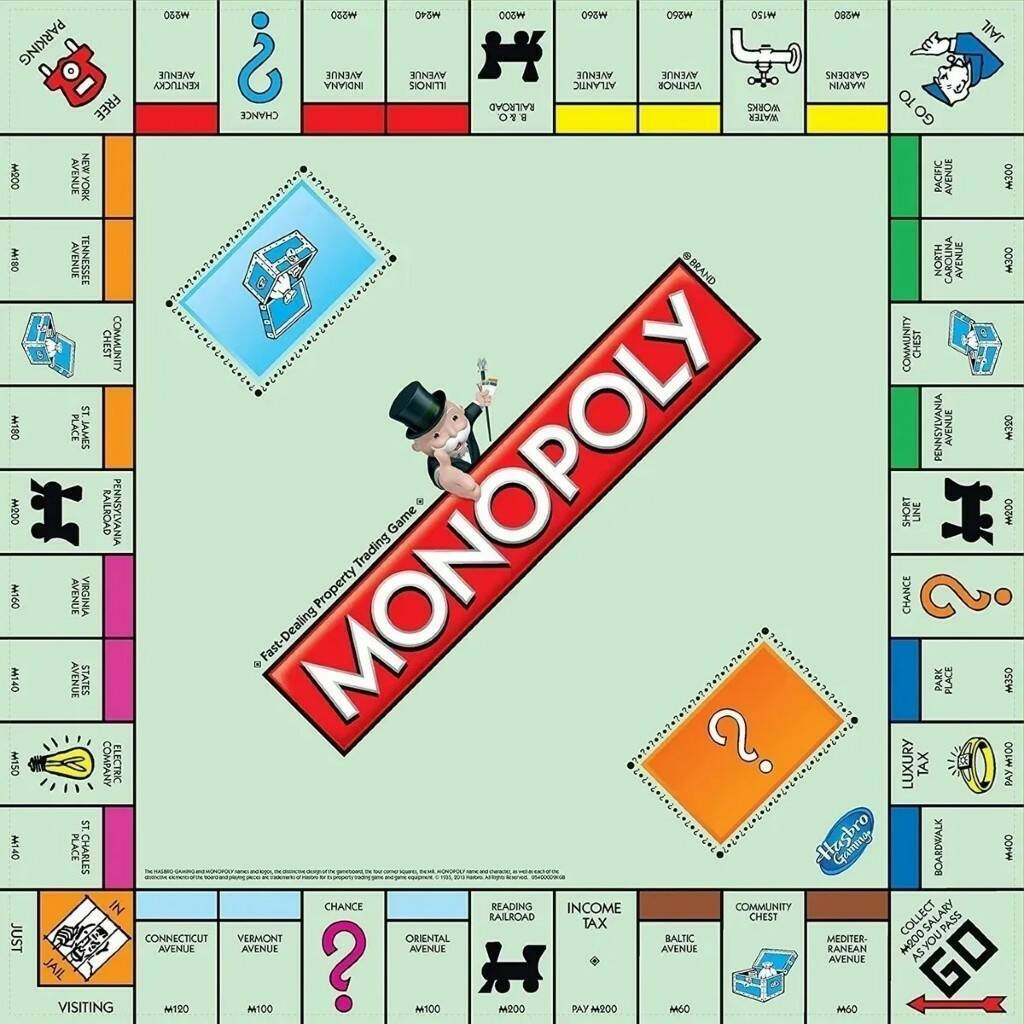
\includegraphics[width=0.6\linewidth, keepaspectratio]{img/momopoly_field}
		\end{center}
		\caption{Поле <<Монополии>>}
	\end{figure}

	Передвижение фишек по карте естественно моделировать конечной дискретной цепью маркова, см. рис.\ref{pic:prob_distr_stoch} . В ней имеется 40 состояний-клеток в соответствии с игровым полем:
	
	\begin{itemize}
		\item 22 клетки улицы
		\item 4 клетки вокзалов
		\item электростанция и водопровод
		\item две клетки налогов -200 и -100
		\item 6 клеток "Шанс"
		\item стартовая клетка, бесплатная парковка и экскурсия(тюрьма), "идти в тюрьму" 
	\end{itemize}
	
	Вероятности переходов из данного состояния соответствуют вероятностному распределению суммы очков при бросания двух шестигранных костей, см. рис.\ref{pic:prob_distr_stoch}  (здесь пренебрегаем правилом запрета выкидывания дублей).Единственную особенность имеет состояние <<иди в тюрьму>>, которое ведёт только в $\ldots$ клетку тюрьмы.
	
	\begin{figure}[h]
		\subfigure[Стохграф игры]{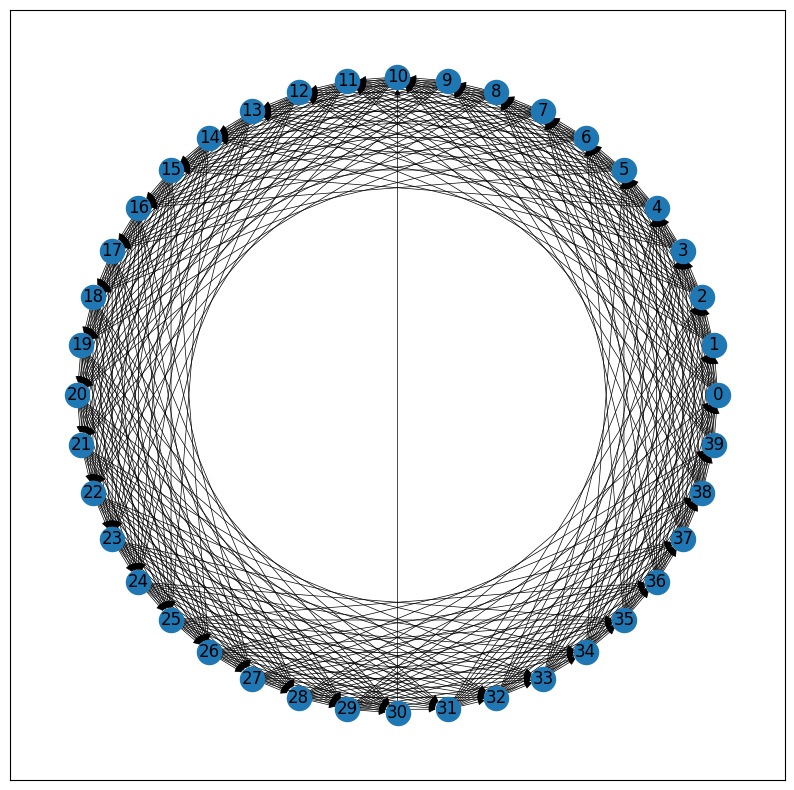
\includegraphics[width=0.49\textwidth, keepaspectratio]{img/chains_graph}}
		\subfigure[Вероятностное распределение кубиков]{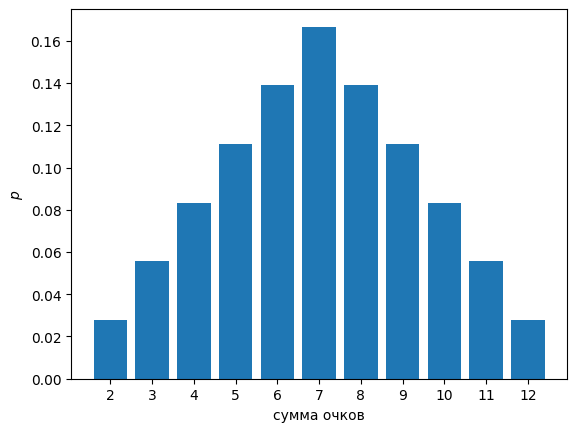
\includegraphics[width=0.49\textwidth, keepaspectratio]{img/dices_distr}}
		\caption{}\label{pic:prob_distr_stoch}
	\end{figure}

	Очевидно, что данная цепь является \textit{эргодической}, что значит существование единственного стационарного распределения, к которому сходится любое начальное распределение по состояниям цепи. Из свойств стохастической матрицы нетрудно понять, что это распределение --- дискретное равновероятное по всем состояниям цепи, т.е. вероятность находится в любом состоянии есть $\dfrac{1}{40} = 0.025$. Вместе с \textit{ЗБЧ для дискретных цепей}, т.е. того факта, что доля попаданий в данное состояние за $N$ шагов сходится по вероятности к стационарному распределению данного состояния $\sum_{i = 1}^N \mathit{1}\{X_i = k\} \to p_k$, мы можем позволить себе руководствоваться лишь найденным стационарным распределением состояний, т.к. именно оно определяет игру в среднем. На малых же интервалах ходов можно и нужно руководствоваться локальным расположением на поле и локальной ситуацией в клетках, но такой анализ совершенно не имеет значения для глобального исхода и общего понимания принципов игры.
	
	\subsection*{Кредитные риски}
	
	Итак, выяснив, что наши шансы оказаться в той или иной клетке поля на больших интервалах времени имеют дискретное равномерное распределение, пора вспомнить, что оно определяет вероятностное распределение случайной величины прибыли, получаемой от недвижимости игроков, карточек <<Шанс>>, клеток налогов, выходов из тюрьмы и прохода полного круга по полю игры. 
	
	Доход от \textit{прохода полного круга} в $200$ \sout{M} предлагается внедрить, как доход в $+5$ \sout{M} от каждой клетки, кроме клетки \textit{<<иди в тюрьму>>}, от неё доход будет $-50$ \sout{M} (стоимость выхода из тюрьмы по правилам).
	
	Далее, имеется \textit{16 карточек <<Шанс>> и <<Общественная казна>>}, со своим распределением дохода и убытков (здесь не учитывается, что эти карточки могут не подмешиваться обратно в общую колоду). Более того, т.к. существуют карточки, результат которых зависит от сложившейся игровой ситуации и количества игроков, то оценка рисков в данном месте вообще говоря должна проделываться на месте. 
	
	Доходы от \textit{собственности} также меняются со временем игры, зависят от типов недвижимости и, например, от сбора полного цветового комплекта. От каждой клетки чужой недвижимости я плачу ренту, от каждой клетки своей недвижимости я получаю  $\text{ренту} \times (N - 1)$, где $N$ ---  общее количество игроков.
	
	Т.о. игрок владеет полной информацией о распределении своей прибыли и соответствующих характеристиках этого распределения. Также важно помнить, что по ходу игры это распределение будет меняться.
	
	\section{Принципы принятия решений и управления недвижимостью}
	
	\subsection*{Вводные слова}
	
	Большую часть времени агенты просто путешествуют по игровому полю, но возникают моменты, когда им нужно принять решение, влияющее на дальнейшее развитие событий. Принципы, которым следует игрок в данных ситуациях, должны исходить из знания о вероятностных свойствах игры, текущей финансовой ситуации и степени неприятия риска.
	
	Для победы в игре необходимо обанкротить других игроков и не обанкротиться самому. Т.о. необходимо проанализировать источники доходов и расходов для игроков. Их можно поделить на \textit{внутриигровые}, т.е. связанные с карточками <<Шанс>>, проходом поля <<Старт>> и т.п., а также на \textit{трансигровые}, т.е. связанные с попаданием на владеемую собственность и движением средств между игроками. Как можно видеть из структуры трансигровых расходов (см. пред. раздел), их сумма по всем игрокам равна нулю, т.е. при владении недвижимостью кто-то всегда обогащается за счёт других. Именно этот источник является ключевым в игре.
	
	\subsection*{Стратегия}
	
	Исходя из всего вышесказанного, можно заключить, что всё, что делает игрок, --- это решает задачу управления риском и задачу размещения ресурсов. Поэтому далее можно брать хоть нормативные документы по управлению риском компании \texttt{Alphabet} или методичку из \texttt{Morgan Stanly}. Т.к. я не владею достаточной степенью знания для уверенного продолжения данного раздела, то все мои дальнейшие советы прошу воспринимать лишь как одну из возможных стратегий поведения. Т.о. игрок может исходить из следующих соображений при принятии решения:
	
	\begin{enumerate}
		\renewcommand{\theenumi}{\Roman{enumi}}
		\item \textbf{Любое действие игрока не должно уменьшать его матожидание прибыли}. Например, если игрок встал на свободную недвижимость, то приобретя её, он обязательно увеличит свой ожидаемый доход от игры. Единственное, что может остановить его в такой ситуации --- это недостаточное количество денежных средств или их такое количество, что риск обанкротиться после покупки в ближайшее время велик для данного игрока (об этом ниже). При данном развитии, недвижимость будет выставлена на аукцион и в любом случае будет приобретена, что также должно учитываться игроком.
		
		 Другой пример: застройка улиц полного цветового комплекта при достаточном уровне резерва на случай убытков. Пока такой возможности нет, игрок может вкладывать деньги только при попадании на свободную собственность. Когда же есть возможность строить дома, то появляется дилемма: либо вложить ограниченные средства сейчас, либо понадеяться на удачу и подождать попадания на свободную собственность, не тратясь. Конечно можно посчитать, сколько шагов пройдёт для достижения хорошей вероятности попадания на свободную клетку (подойдёт геометрическое распределение для одного состояния), учесть, что на неё может попасть другой игрок и сравнить это с прибыльностью от вложения средств в дома, но почти всегда лучше делать последнее, ведь в этом и смысл игры --- быть монополистом и срывать с этого куш.
		 
		 Третий пример: обмен собственностью в игре всегда должен быть взаимовыгодным, т.е. у обоих агентов при сделке матожидание не должно уменьшаться (или игрок может допустить небольшое уменьшение за счёт дополнительной денежной выплаты для его целей). При этом также стоить учитывать не только изменение своего матожидания из-за простого обмена, но также и последующих действий, например, в результате другой игрок может собрать весь цвет и сразу же застроить улицы, что резко отразиться на вашем матожидании. Более того, если его матожидание прибыли положительно, то в среднем он будет зарабатывать и продолжать застройку. Стоит прикинуть эти варианты перед сделкой.
		 
		 \item \textbf{Каждый игрок определяет, что есть для него риск и каковы его допустимые пределы}. Пример простой процедуры может выглядеть так: пусть после совершения некоторой операции у меня осталась сумма $S$. Тогда мой риск обанкротиться в ближайше время есть $F(-S)$, где $F(x)$ --- функция распределения моей прибыли. Решение о том, является ли такой риск допустимым, определяет судьбу данной операции (если называть вещи своими именами, то это есть не что иное, как метрика риска $VaR$).
		 
		 \item \textbf{Другие факторы}. Например, нежелание игрока затягивать игру, утруждать себя умозаключениями и т.п. Каждый заполняет данную графу в индивидуальном порядке.
	\end{enumerate}
	
	\subsection*{Оптимальный менеджмент}
	
	Изложенные руководящие принципы можно выразить в виде алгоритма, решающего задачу оптимизации матожидания прибыли агента, оставаясь в допустимых пределах риска. На текущий момент решение данной задачи остаётся за рамками данной работы.
	
	\section{Замечания к изложенной теории}
	
	Хочется обратить внимание на то, что в работе не делается попытка провести комплексный теоретико-игровой анализ. Конечно, возможно представить себе бесконечное дерево динамической игры, в котором существуют равновесия и оптимальные стратегии, но всё-таки данный подход непривлекателен как с математической точки зрения, так и с вычислительной. Я не представляю получения продуктивного результата в данном направлении. Напротив, анализ игры в среднем очень продуктивен и естественен. В такой модели даже жадные стратегии приводят к хорошим результатам. Более того, как упоминалось, возможно просчитывание наперёд и оптимизация управления ресурсами.
	
\end{document}








